\section{Introduction}
\label{sec:intro}

\subsection{A Great Theorem}
The Gauss-Bonnet theorem relates the curvature, a local property, of a surface
to the Euler characteristic, a global property. In symbols 

\begin{equation}\label{eqn:g-b-noboundary}
		\int_MK dA =2\pi \chi(M)
\end{equation}
where $M$ is a smooth surface in $\RR^3$ without boundary, $K$ is Gaussian curvature
and $\chi(M)$ is the Euler characteristic of $M$.
The theorem is a bridge between many ideas that may
seem separate at first, see \figref{bridge}. 




\begin{figure}[htb]
\centering
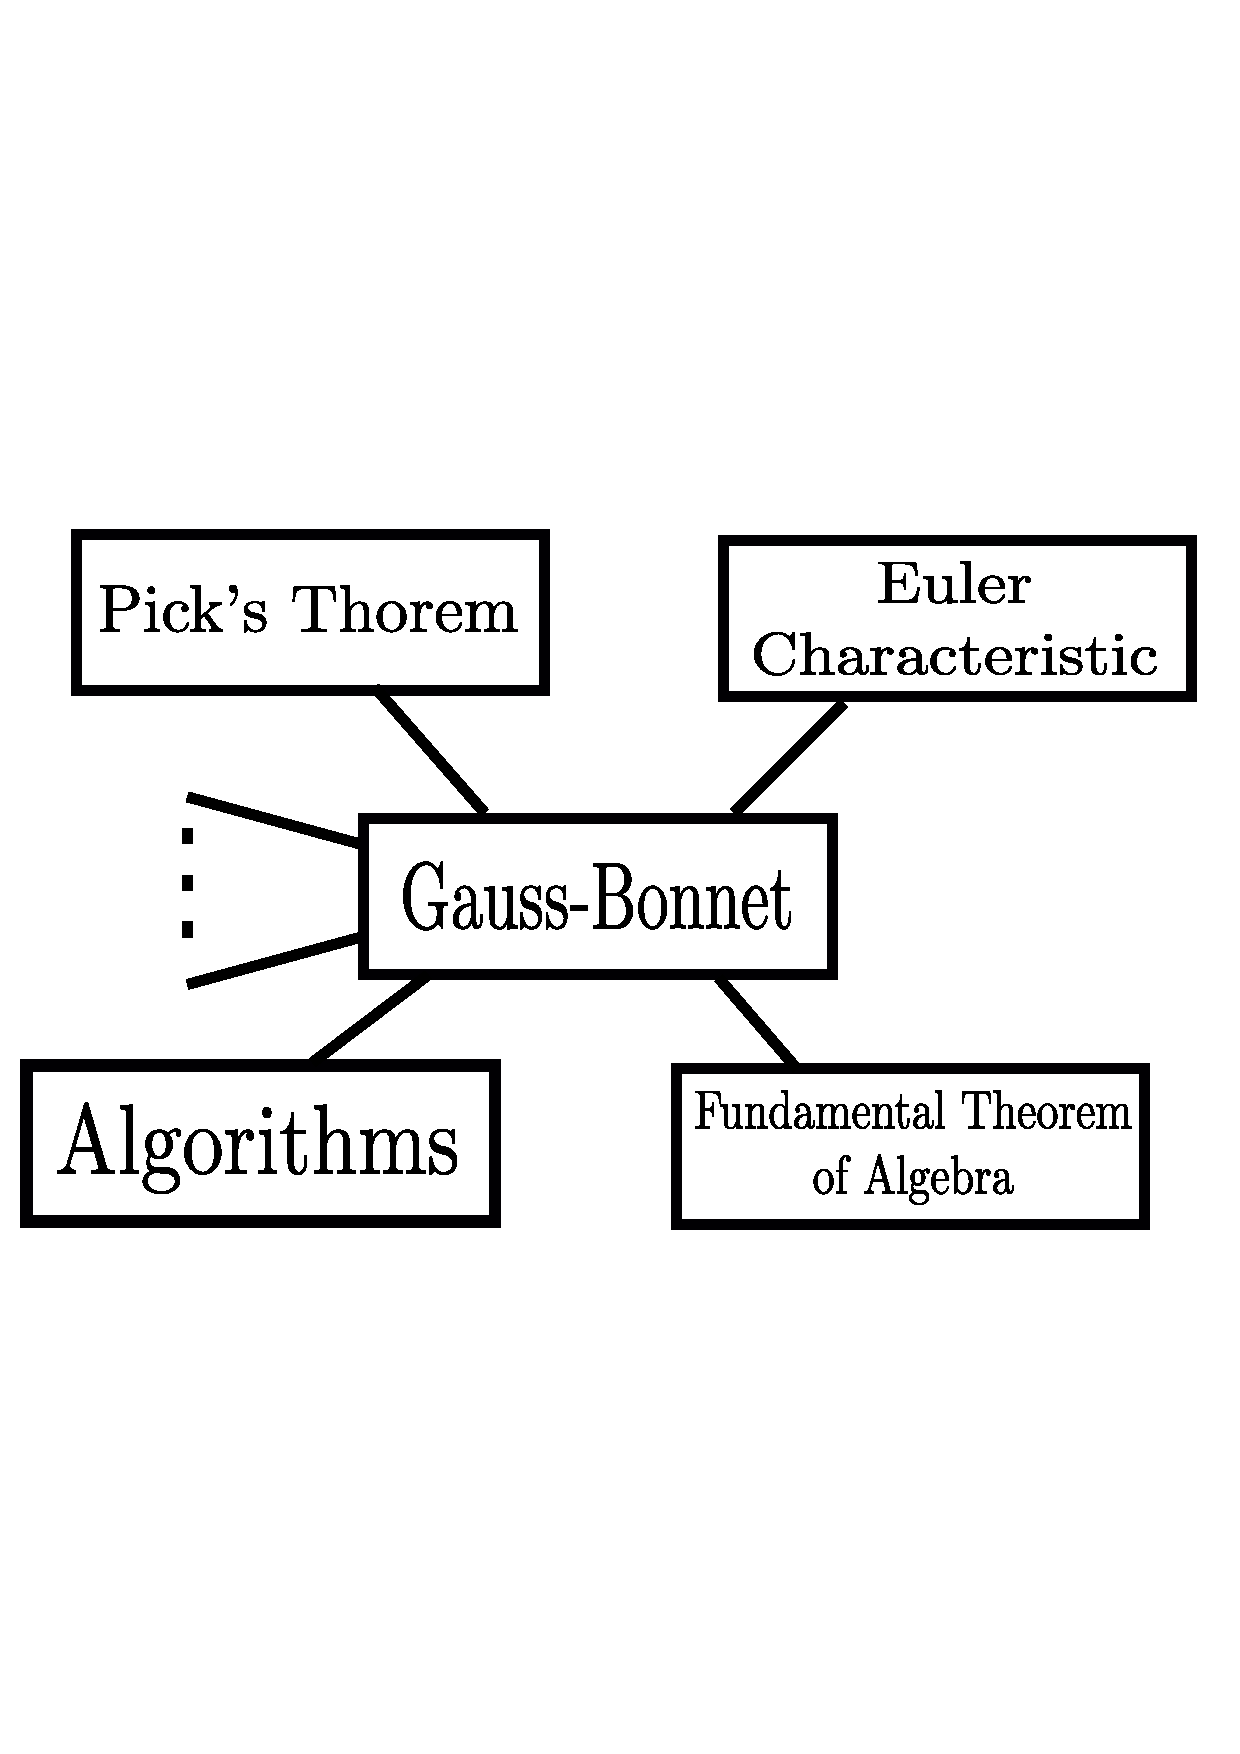
\includegraphics[width=.3\textwidth]{curvature/bridge}
\caption{The Gauss-Bonnet theorem is a star.}
\label{fig:bridge}
\end{figure}

In the book \emph{Using the Borsuk-Ulam Theorem}
\cite{jm08},
Matou\v{s}ek states that a theorem is a great theorem if there are
\begin{enumerate}[(1)]
\item several different equivalent versions,
\item many different proofs,
\item a host of extensions and generalizations, and
\item numerous interesting applications.
\end{enumerate}

By this criteria, the Gauss-Bonnet theorem is a great theorem.
For (1), six\todo{verify} different versions of the theorem are discussed
in \cite{wu_historical_2008}. 
In addition to the version for smooth surfaces given in \eqnref{g-b-noboundary},
we highlight
 several discrete versions for triangulated surfaces. 
  




 
 
As for (2), several fundamentally different proofs exist.  
One common approach is to first prove the theorem for simply connected domains
with boundary, then triangulate a surface and add up the contribution from each triangle.
However, this proof seems to lack a geometric intuition that other proofs provide. \cite{wu_historical_2008},
A second commonly seen proof is to use Stokes theorem  \cite{doc76,pressley_elementary_2010}.
Many other proofs exist \cite{guillemin_differential_2010,levi-bicycle,grinfeld_introduction_2013}.


For (3), the theorem has been generalized in many ways.
The two notable examples are the Chern-Gauss-Bonnet theorem\cite{chern_simple_1944} and
the Atiyah–Singer index theorem is an example  \cite{atiyah_index_1963}.
A generalization to higher dimensions \cite{guillemin_differential_2010}.


As for (4), applications, 
seven are given in \cite{doc76}.
For applications to physics see \cite{tirado-physics-apps,gibbons_applications_2008}.
This work provides many examples related to the algorithms and combinatorics. 
I hope that the number of applications continues to grow,
please share any that you feel
ought to be included\footnote{\text{mccoy2ba@jmu.edu}}.


\subsection{Simple Polygons}
\label{sec:warm-up}

Some of us may remember the following special case
of the Gauss-Bonnet theorem from middle school geometry.
Consider a simple polygon $P$, an example is shown in \figref{polygon}.

 \begin{figure}[htb]
         \centering
          \begin{subfigure}[b]{0.30\textwidth}
      		   \includegraphics[width=\textwidth]{background/blank-polygon}
    		    \caption{A simple polygon.}
 		 \label{fig:polygon}
	 \end{subfigure}
	 \hspace{.5cm}
	 \begin{subfigure}[b]{0.25\textwidth}
       		  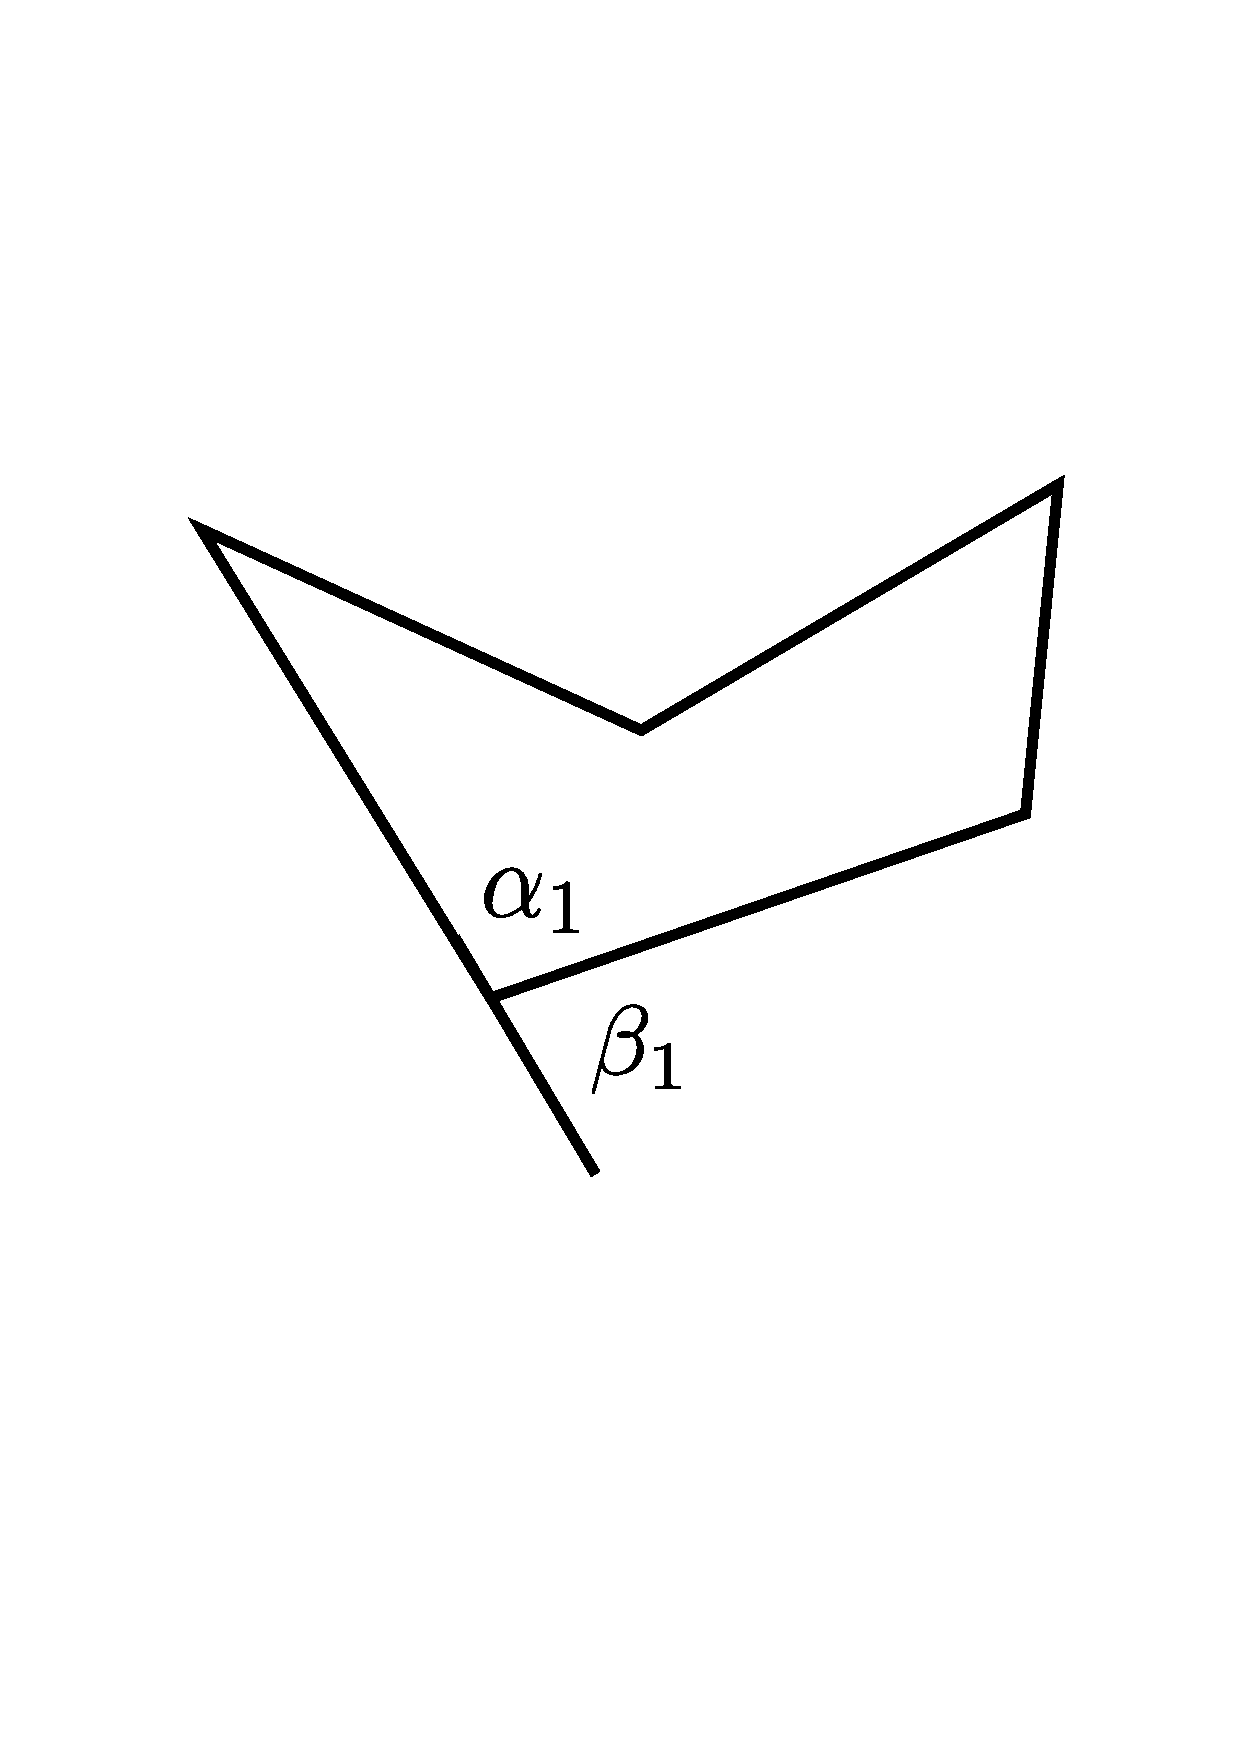
\includegraphics[width=\textwidth]{background/interior-exterior}
     		    \caption{Angles}
 		 \label{fig:interior-exterior}
       \end{subfigure}
        \hspace{.5cm}
     \begin{subfigure}[b]{0.27\textwidth}
       		  \includegraphics[width=\textwidth]{background/exterior-angles-polygon}
       		  \caption{Exterior angles.}
       		   \label{fig:exterior-angles}
         \end{subfigure}
		\caption{(\subref{fig:polygon}) A simple polygon $P.$
		(\subref{fig:interior-exterior}) The interior and exterior angles formed at a vertex.
 		 (\subref{fig:exterior-angles}) The sum of the exterior angles of a simple
		polygon is $2\pi$. Here
		$\beta_1+\beta_2+\beta_3+\beta_4+\beta_5=2\pi$ note that $\beta_4$ is negative.
 		\label{fig:simple-polygon}}
 \end{figure}

If we extend one of the sides of $P$ two complementary angles appear.
The angle inside $P$ is the \EMPH{interior} angle and the complement 
is the  \EMPH{exterior angle}. An example is shown in \figref{interior-exterior}.
We differentiate between turning left and right.
Vertices with interior angles  greater than $\pi$ are called \EMPH{reflex}, see \figref{exterior-angles}. 
At reflex vertices exterior angle is negative.



We now state a simple version of the Gauss-Bonnet theorem \cite{gottlieb_all_1996,polya_elementary_1954},

\begin{theorem}[Gauss-Bonnet for Polygons in the Plane]\label{thm:simple-bonnet}
Let $P$ be a simple polygon in the plane with $n$  vertices,
interior angles $\{\alpha_1,\alpha_2,\ldots,\alpha_n\}$
and exterior angles $\{\beta_1,\beta_2,\ldots,\beta_n\}$ then
$$\sum_{i=1}^n\beta_i=2\pi$$
and 
$$\sum_{i=1}^n\alpha_i=\pi(n-2).$$
\end{theorem}


\begin{proof}

	We traverse a polygon and rotate $\beta_i$ at each vertex
	when we get back to where we started we will have preformed 
	one complete revolution so $\sum_{i=1}^n\beta_i=2\pi.$
	The exterior angles are complementary to the interior angles
	so for each $i$ we have $\beta_i=\pi-\alpha_i$  and using the first
	part of the theorem,  we have
	$\sum_{i=1}^n(\pi-\alpha_i)=n\pi -\sum_{i=1}^n\alpha_i=2\pi$. 
	Solving for $\sum_{i=1}^n\alpha_i$ gives the second part of the theorem.

\end{proof}
No matter how we position the vertices of our polygon,
if the boundary of the polygon stays closed and simple,
the sum the exterior angles will be $2\pi$.
Even this simple version of the Gauss-Bonnet theorem has powerful
consequences, as we now see in our first application, a proof of Pick's Theorem.





\subsection{Pick's Theorem}
\label{sec:pick}

Pick's Theorem gives a formula for the area of a polygon
in the plane with vertices on the lattice $\ZZ^2$ \cite{og-pick}.
We give a proof originally due to Blatter \cite{blatter_another_1997}
and restated by Tabachnikov  \cite{tabachnikov_proofs_2014}.

\begin{theorem}[Pick's Theorem]\label{thm:pick}
Let $P$ be a simple polygon in the plane with vertices on the lattice $\ZZ^2$,
let $I$ be the number of lattice points inside of $P$, let $B$ be the number
of lattice points on the boundary of $P$ and let $A$ denote the area of $P$.
Then, 
$$A=I+\frac{B}{2}-1.$$
\end{theorem}
See \figref{picks} for an example.

 \begin{figure}[htb]
         \centering
         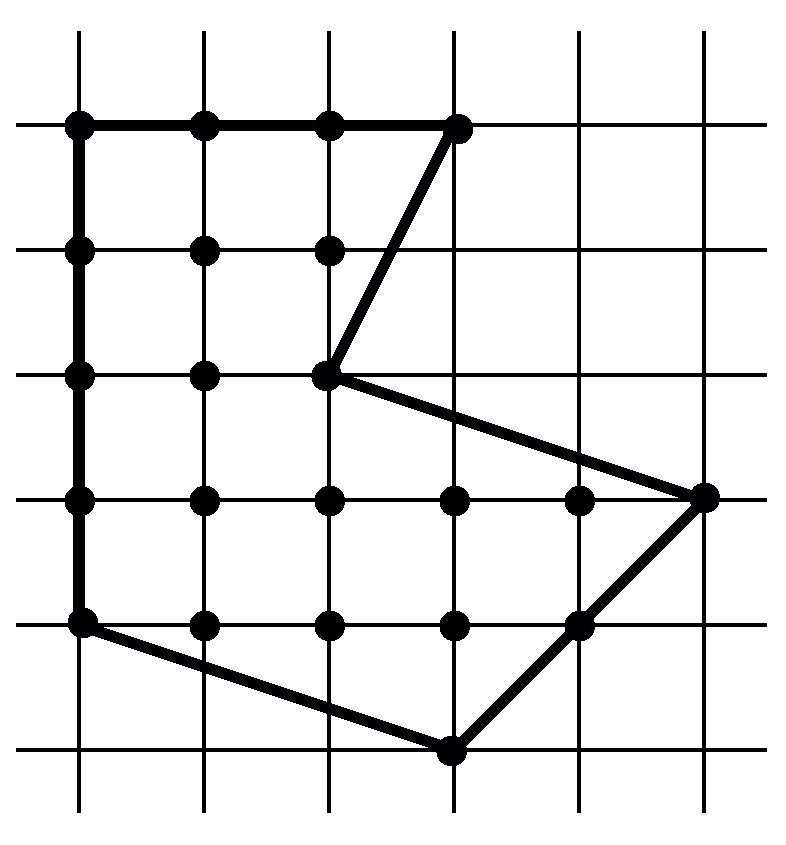
\includegraphics[width=5cm]{pick}
	\caption{A polygon with vertices on the lattice. 
	There are 10 interior vertices and 12 vertices on the boundary.
	By Pick's theorem the area of the polygon is $10+\frac{12}{2}-1=15.$
	\label{fig:picks}}
 \end{figure}
 
\begin{proof}
	Put a unit volume ice cube at each lattice point in the plane and let the ice melt.
	The water will evenly cover the plane with the amount of water inside the polygon 
	equal to its area.
	
	Consider a edge on the the polygon. The amount of water that flows
	into to polygon across this edge equals that amount of water that flows out of the polygon
	across this edge by symmetry. This is because the edge connects two lattice points,
	for each point the contributes flow across the edge in one direction there is a symmetric
	point that contributes and equal amount of flow in the opposite direction.
	So, the total flow across each edge is zero and
	the  amount of water inside the polygon comes from interior cubes and the lattice vertices
	of the polygon.
	
	Each interior lattice point contributes one unit of water. 
	Each lattice point on an edge, half of the water flows into the polygon and
	half flows outside of the polygon.
	Let $\alpha_i$ denote the interior angles at each vertex.
	Each vertex contributes $\frac{\alpha_i}{2\pi}$ units of water to the area.
	By the Gauss-Bonnet theorem, \thmref{simple-bonnet}, the sum of the interior
	angles is $\pi(n-2)$. Thus, the vertex points contribute a total of 
	$$\frac{\pi(n-2)}{2\pi}=\frac{n}{2}-1.$$
	The theorem follows.

\end{proof}




